%!TEX root = ../thesis.tex
\chapter{Software Architecture}
\label{chap:architecture}

In this chapter, the composition of the system is described with more detail.One of the challenges when developing SAJaS wasdeciding how to implement assynchronous JADE-based features in a tick-based environment. This is described in Section \ref{sec:agentexecution}. Following it the definition of the architecture of the system in the form of conceptual diagrams. Closing this chapter is a discussion on the extension perspectives of the system.

\subsection{Agent Execution}
\label{sec:agentexecution}

% Agent execution in JADE and Repast
JADE agent execution can be concurrent and parallel, since JADE supports distributed and multi-threaded agent systems. Agent execution in Repast, on the other hand, is not concurrent. Repast uses a time-share type of execution, granting each agent the right to perform its tasks until they finish them, in sequence, but in no particular order.

% Agent execution in the API
When integrating agent behaviours in \apiname{}, including those related with interaction protocols, it was necessary to make adaptations to JADE behaviours implementation, in order to take Repast's concept of time into account. Even though a local application can take advantage of direct method invocation, for the sake of compatibility with JADE, communication in \apiname{} is also made asynchronously.

Figures \ref{fig:com-example-jade} and \ref{fig:com-example-repast} represent a scenario where two agents send a message to a third one who then replies. In Repast (Fig. \ref{fig:com-example-repast}), messages are delivered to agent C's message queue, and processed only in C's turn. In JADE (Fig. \ref{fig:com-example-jade}), messages can arrive concurrently. Their arrival triggers an event and they are processed right away. In this case, agent C handled the messages as they arrived and issues the respective replies.

\begin{figure}[h]
	\centering
	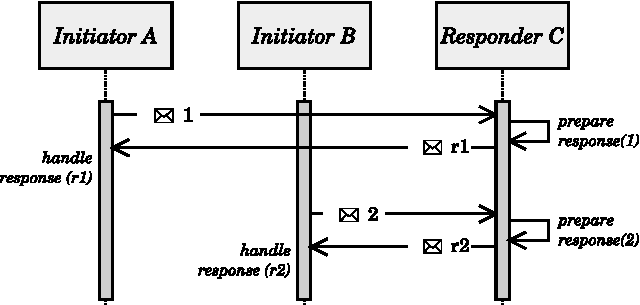
\includegraphics[width=3.0in]{figures/tickExample2.pdf}
	\caption{
		Communication example in JADE. Agents are executed concurrently or in parallel. 
	}
	\label{fig:com-example-jade}
\end{figure}

\begin{figure}[h]
	\centering
	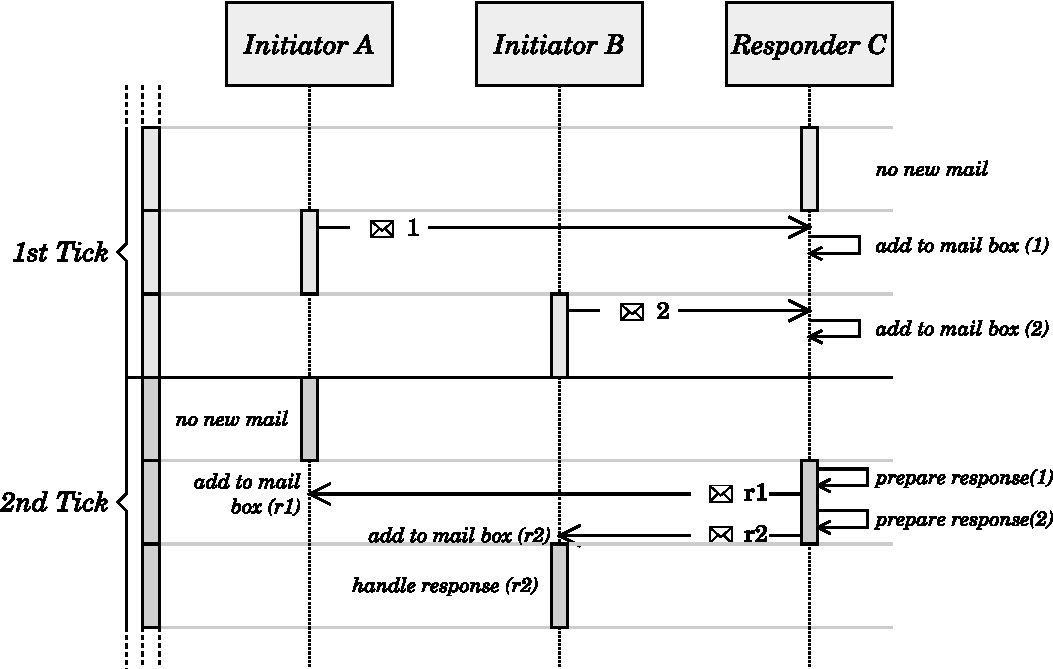
\includegraphics[width=3.8in]{figures/tickExample.pdf}
	\caption{
		Communication example in Repast using \apiname{}.
	}
	\label{fig:com-example-repast}
\end{figure}

While the diagram above represents the agents as scheduled objects, their behaviours are the ones actually being scheduled. It is worth noting that the order by which Repast executes each scheduled behaviour is unpredictable. In fact, it is not guaranteed that all the behaviours of a single agent are executed consecutively. This is the expected execution when working with Repast as well as with JADE (given its multi-threaded nature) and it is up to the programmer to ensure that the application does not rely on the order of execution.

\subsection{Architecture}

Figure \ref{fig:arch} illustrates the details of \apiname{}'s architecture. Most concepts represented in this diagram are present in JADE, namely the Agent, ACL Message, Behaviour, MTS and DF service.

An agent in \apiname{} contains a MessageQueue and a set of Behaviours. These have access to the agent who owns them and to its MessageQueue. A behaviour that implements an interaction protocol makes use of MessageTemplates. These are used to retrieve relevant messages in each step of the protocol. The MessageTemplates are updated while the protocols go through their different states.

The DFService, as described before, provides the yellow page service. Agents can register or deregister themselves in the DF as well as perform searches. While tasks can be performed during agent setup, in runtime they are typically executed inside Behaviours.

To follow JADE-like communication, ACL Messages carry agent identifiers (AID) for senders and receivers. These AIDs are returned by the DF as search results and are resolved to an agent by the MTS when sending a message. In \apiname{} the MTS keeps a mapping of AIDs to agents for easier access.

The ``plug-in points'' of the API are the Agent, the Behaviour and their derived classes. The API also supports direct access to the DFService. In Figure \ref{fig:arch} all protocol definitions are implied by the generic sub-classes ``ProtocolInitiator'' and ``ProtocolResponder''. 

\begin{figure}[h]
	\centering
	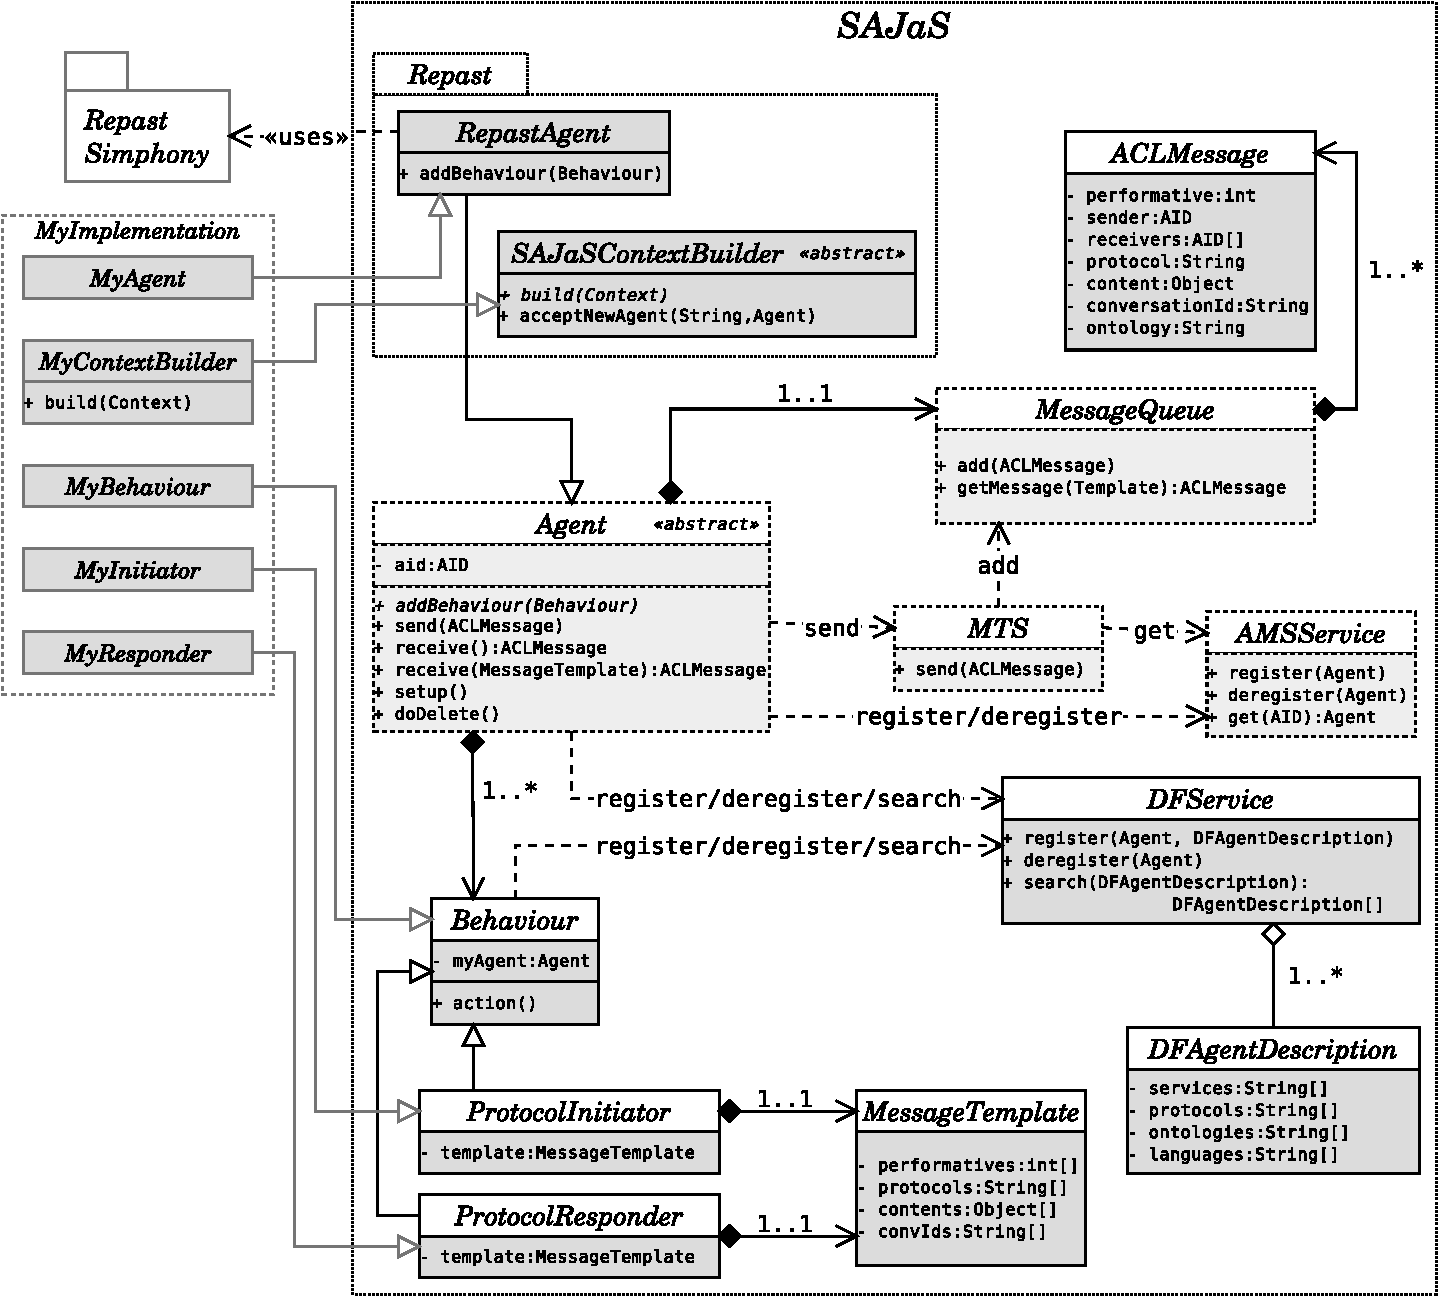
\includegraphics[width=\linewidth]{figures/repacl_arch.pdf}
	\caption{Detailed architecture of \apiname{}. The classes with doted border are internal.}
	\label{fig:arch}
\end{figure}